SpiderMonkey is the JavaScript Engine for Mozilla, an extremely widely
used, security-critical interpreter/JIT compiler.  SpiderMonkey has
been the target of aggressive random testing for many years now.  A
single fuzzing tool, \texttt{jsfunfuzz} \cite{jsfunfuzz}, is
responsible for identifying more than 1,700 previously unknown bugs in
SpiderMonkey \cite{jsfunfuzzbugs}.  SpiderMonkey is (and was) very
actively developed, with over 6,000 code commits in the period from
1/06 to 9/11 (nearly 4 commits/day).  SpiderMonkey is thus ideal for
evaluating how reduction aids localization when using a sophisticated
random testing system, using the last public release of the
\texttt{jsfunfuzz} tool \cite{jsfunfuzz}, modified for swarm testing \cite{ISSTA12}.
Using a set of faults in SpiderMonkey version 1.6 found with random
testing in previous research \cite{PLDI13}, we show that reduction is
essential for localization of bugs found using random testing, and
that the use of reduction is even somewhat more important than the
choice of localization formula.  Note that this is an extremely
challenging setting for spectrum-based localization: randomly
generated successful tests tend to cover a wide variety of behavior,
some of it in a very shallow fashion, which makes distinguishing the
signal of lines covered more frequently in failing tests from general
noise (and particularly the noise of lines that are simply hard to
cover and happen to appear in the failures) very difficult.

\begin{table}
\begin{center}
\begin{tabular}{|c||c|c|c|c|c||c|c|c|c|c|}
\hline

\hline
Bug\# & Revision Fixed &  \#Failures & {\tt diff} size \\
\hline
\hline
{\tt R60} & 1.16.2.1 & 1 & 115  \\
\hline
{\tt R95} & 1.3.2.3.8 & 7 & 111   \\
\hline
{\tt R115} & 1.4.8.1 & 4 & 592   \\
\hline
{\tt R360} & 3.117.2.6 & 3 & 223  \\
\hline
{\tt R880} & 3.17.2.14 & 28 & 272   \\ 
\hline
{\tt R1172} & 3.208.2.63 & 150 & 214  \\
\hline
{\tt R1294} & 3.241.2.1 & 405 & 80  \\
\hline
{\tt R1543} & 3.36.16.1 & 146 & 169  \\
\hline
{\tt R1561} & 3.37.2.1.4.1.2.2 & 2 & 31  \\
\hline
{\tt R1873} & 3.50.2.29 & 1,041 & 56  \\
\hline
\hline
\end{tabular}
\end{center}
\caption{Spidermonkey Bugs}
\label{tab:spiderbugs}
\end{table}


\begin{figure*}[t]
  \centering
  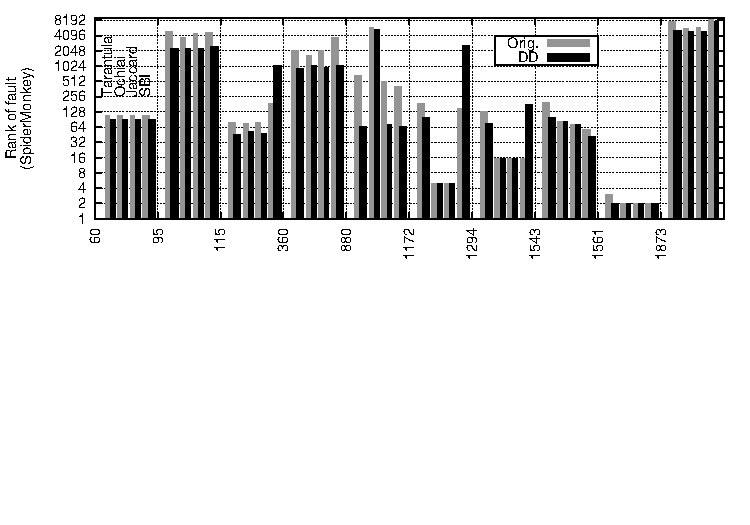
\includegraphics[width=2\columnwidth]{naspidermonkey}
 \vspace{-2.2in}
  \caption{SpiderMonkey Results}
  \label{fig:spidermonkey}

\end{figure*}

Figure \ref{fig:spidermonkey} shows the change in rankings of the
faulty code for 10 SpiderMonkey bugs (Table \ref{tab:spiderbugs}).
These bugs were taken from our PLDI 2013 data set \cite{PLDI13}.  Out
of the 28 bugs studied in that paper we chose 10 random bugs for which, by
hand, we could confirm the true set of faulty lines in the code
commit.  Each bug is identified by the revision number of the commit
in which it was fixed: e.g., R0 maps to revision 1.10.4.1, the first
commit of Spidermonkey changes under consideration. Table
\ref{tab:spiderbugs} shows all bugs studied, the commit version fixing
the bug, the number of failing test cases for that bug (\# Failures),
and the size (in lines) of the fixing commit's {\tt diff}.  The faults
under consideration here are clearly non-trivial (in fact, most fixes
involved changes to multiple source files).  For our localization we
used the original and reduced test cases from PLDI 13 \cite{PLDI13}
plus a set of 720 randomly generated passing tests generated using the same method as in
the original data set.

Across these 10 bugs, the average ranking for the first faulty line
encountered was 1,550.7 without reduction, improving to 994.5 with
reduction.  Reduction improved the localization in 33 cases, with a
minimum improvement of 1 ranking and a maximum improvement of 2,137
positions.  The average improvement was 674 positions.  The results
were unchanged in 7 cases. It is important to note that even with such a challenging setting and real bugs, fault localization with reduction performs better then fault localization without reduction irrespective of formula being used, in worst case it performed as good. It was better to use reduction than to optimally (from worst to
best) switch formula for 5 of the 10 bugs; it was better to switch
formula in 4 cases, and in one case both methods gave the same result.
While the results show that reduction was extremely effective in
improving localization, it is also true that the localization was
\emph{still not very helpful} in many of these cases, considering absolute pessimistic rank as success criteria.  Of course,
SpiderMonkey 1.6 has over 80KLOC, and even reduced failing tests
typically executed over 8,000 lines of code, so a ``poor''
localization may be useful in such a large fault search space.  For 6
of the 10 bugs, all scores after reduction gave the fault a ranking of
128 or better.  We also suspect that experienced developers could dismiss
at least some of the lines in the rankings immediately, as we discuss
next.

In order to expand on how reduction improves localization, we examine in more detail the bug
we call ``R1543,'' fixed by commit 3.36.16.1, and its Tarantula
localization.  In our experiments, there were 146 test cases that
failed due to bug R1543.  The relevant commit contains three kind of
changes: (1) a rename refactoring, (2) a refactoring for readability,
and (3) the actual fault fix.  The fault is in {\tt jsexn.c}, in the
function {\tt Exception}. Comparing diffs of R1542 and R1543 we were
able to identify lines 583, 587, 589, 590 and 594 as the actual faulty
code. Before reduction, these lines (all with suspiciousness 0.716605)
had rankings from 191 on (ranking is arbitrary among buggy lines of
same suspiciousness).  After reduction, the rankings improved to start
at 98.  The suspiciousness values of faulty lines, as discussed in Section
\ref{formal}, remained unchanged.  However, many higher ranked non-faulty lines
became less suspicious after being removed from failing tests.  The
average coverage for an unreduced failing test was 11,461 lines, which
decreased to 8,349 (an average decrease of 3,112 lines) after reduction.

When we looked at the lines ranked before the faulty lines, we found
that 70 lines in unreduced ranking and 56 lines in post-reduction
rankings were assigned suspiciousness values of 1.0. These lines
execute only in failing test cases. Our further investigation suggests
that many of these lines are actually failure handling and reporting
code.  For example, 23 of the highly ranked lines for R1543 are part
of the functions {\tt my\_ErrorReporter} and {\tt Quit} in {\tt js.c},
clearly failure handling and reporting code that would not slow an
experienced SpiderMonkey developer in reaching the actual fault.  We
found such failure handling and reporting code in highly ranked lines
for other bugs as well (finding them is fairly easy, as they have
suspiciousness 1.0 by Tarantula).  While many lines that are not such
obviously non-faulty code remain for many SpiderMonkey bugs, this
suggests a follow-on to Parnin and Orso's experiments \cite{AutoHelp}:
while they included some more experienced developers in their study,
they did not investigate how developers highly skilled with \emph{a
particular code base} use fault localization.  We speculate that while
the raw rankings for many SpiderMonkey bugs are not very high, some of
these results could be more useful than is apparent, in the hands of
expert developers.  Such users are the most likely eventual industrial
adopters of localization, we believe, for complex projects where
debugging can be extremely difficult and time consuming and aggressive
automated testing is used.\footnote{We the authors have submitted
Chrome JavaScript engine bugs found during testing research and seen
that it may take months to understand and fix some complex failures.}
